% main.tex --- 修論用アブスト(2ページ二段組, LuaLaTeX)
\documentclass[a4paper,10pt,twocolumn]{ltjsarticle}

\usepackage[haranoaji]{luatexja-preset}
\usepackage[top=20mm,bottom=20mm,left=20mm,right=20mm]{geometry}
\usepackage{graphicx}
\usepackage{booktabs}
\usepackage{siunitx}
\usepackage{caption}
\usepackage{titlesec}
\usepackage[hidelinks]{hyperref}
% 2ページ制約のため,参考文献は簡潔表示(URL/DOIは省略)
\usepackage[
  backend=biber,
  style=numeric,
  sorting=none,
  maxnames=3,
  minnames=1,
  giveninits=true,
  doi=false,
  url=false,
  isbn=false,
  eprint=false
]{biblatex}

% meta.tex --- 論文メタ情報(ここだけ編集すればOK)
% 全角数字にしたい場合は「2025」のように入力してください。

% ===== 表紙に出る情報 =====
\newcommand{\ThesisYearLabel}{2025年度修士論文}
\newcommand{\ThesisTitle}{HAR不確実度に基づくBLE広告間隔の適応制御に関する研究}

\newcommand{\University}{中部大学大学院}
\newcommand{\GraduateSchool}{工学研究科}
\newcommand{\Department}{情報工学専攻}
\newcommand{\Course}{博士前期課程}

\newcommand{\AuthorFamily}{萩原}
\newcommand{\AuthorGiven}{圭島}

\newcommand{\AdvisorFamily}{木村}
\newcommand{\AdvisorGiven}{秀明}

% ===== PDFの「修士論文題目」ページ(要旨ページ)に出る情報 =====
\newcommand{\AbstractDepartment}{情報工学専攻}

\addbibresource{references.bib}

% ページ番号は出さない
\pagestyle{empty}

% 段組間の余白
\setlength{\columnsep}{7mm}

% 段落
\setlength{\parindent}{1\zw}
\setlength{\parskip}{0pt}

% 見出し: "1. はじめに" 形式(太字は避け、サイズで区別)
\titleformat{\section}[runin]{\normalfont\large}{\thesection.}{0.6em}{}
\titlespacing*{\section}{0pt}{0.7\baselineskip}{2\zw}
\titleformat{\subsection}{\normalfont\large}{\thesubsection}{0.6em}{}
\titlespacing*{\subsection}{0pt}{0.4\baselineskip}{0.2\baselineskip}

% 図表キャプション: "図 1 タイトル" / "表 1 タイトル"(コロン無し)
\DeclareCaptionLabelFormat{nonspace}{#1#2} % 図2 / 表1(スペースなし)
\captionsetup{labelformat=nonspace,labelsep=space}
\captionsetup[figure]{name=図,position=bottom}
\captionsetup[table]{name=表,position=top}

% 参照(図/表)
\newcommand{\figref}[1]{図~\ref{#1}}
\newcommand{\tabref}[1]{表~\ref{#1}}

% 記号(本文と衝突しない表記に統一)
\newcommand{\Pout}{P_{\mathrm{out}}}
\newcommand{\epsout}{\epsilon}
\newcommand{\rhohundred}{\hat{\rho}_{100}}

% [1][2] 形式の引用
\DeclareCiteCommand{\scite}
  {}
  {\mkbibbrackets{\usebibmacro{citeindex}\usebibmacro{cite}}}
  {}
  {}

% 浮動体の間隔を詰めて2ページに収めやすくする
\setlength{\textfloatsep}{8pt plus 2pt minus 2pt}
\setlength{\intextsep}{6pt plus 2pt minus 2pt}
\setlength{\floatsep}{6pt plus 2pt minus 2pt}
\setlength{\dbltextfloatsep}{8pt plus 2pt minus 2pt}
\setlength{\dblfloatsep}{6pt plus 2pt minus 2pt}

% 文献(2ページ制約のためコンパクトに)
\renewcommand*{\bibfont}{\scriptsize}
\setlength{\bibitemsep}{0pt}

\begin{document}

\twocolumn[
\begin{center}
  {\Large \AbstTitle\par}
  \vspace{1mm}
  {\normalsize \AbstAuthor\quad \AbstAdvisor\par}
  {\normalsize \AbstAffiliation\par}
  \vspace{3mm}
\end{center}
]

\section{はじめに}
ウェアラブル等のエッジ端末における行動認識(Human Activity Recognition; HAR)では,推論と通信が電力消費を支配しやすい.Bluetooth Low Energy(BLE)広告\scite{BluetoothSIGCore52}は簡便なブロードキャスト手段だが,スマートフォン受信(スキャン)が非理想であるため,固定広告間隔では遅延分布の裾が悪化し得る\scite{Luo2021BLENeighborDiscoverySurvey}.本研究は,HARの不確実度に応じてBLE広告間隔を適応させ,QoS制約$\Pout(\tau)\le\epsout$($\tau=\SI{1}{\second}$,$\epsout=0.1$)の下で送信側消費を抑えることを目的とする\scite{Schrader2016BLEPower,Chen2020BLEPowerMgmt}.

\par
本稿では,意思決定に基づく省電力ビーコニング\scite{Fujisawa2024BLEBeaconing}に着想を得つつ,広告間隔$\SI{100}{\milli\second}$/$\SI{500}{\milli\second}$の2値切替を実装し,TX/TXSD/RXの三ノード計測により電力とQoSを同一試行で評価した.

\section{提案手法}
不確実度の指標にはエントロピー\scite{shannon1948}等が知られるが,実装上は計算量や確率の校正(calibration)\scite{guo2017calibration}の影響が重要である.本研究ではHARモデルの出力確信度と時系列安定度から通信信頼度指標CCS(Communication Confidence Score)を構成する.CCSに基づいて広告間隔を切り替え,本アブストでは実装の最小構成として$\SI{100}{\milli\second}$と$\SI{500}{\milli\second}$の2値切替方策を扱う.CCSが低い(遷移・不確実)区間では短間隔へ寄せてQoSを守り,それ以外は長間隔へ寄せて平均消費を下げる.評価指標は,送信イベント当たり電荷$q_{\mathrm{event}}$(\si{\micro\coulomb}/event)と遅延指標TLおよび期限超過率$P_{\mathrm{out}}(\tau)$とし,平均電力は補助的に用いる.

\subsection{CCSと2値切替}
CCSは,モデル出力の確信度と,推定ラベルの時間的一貫性(安定度)を合成して定義する.具体例として,確信度と安定度の加重和を用い,閾値とヒステリシスにより状態(ACTIVE/QUIET等)を切り替える.これにより,遷移が多い区間ほど短間隔に滞在し,定常区間は長間隔に滞在する設計とする.

\par
切替が閾値のみに依存すると振動し得るため,ヒステリシスに加えて最小滞在時間を設ける.さらに,受信側のQoS悪化が観測された場合は強制的に短間隔へ退避するフェイルセーフを導入し,制約違反を抑制する.

\section{実験}
計測はTX(DUT),TXSD(電力ロガ),RX(受信ロガ)の三ノード構成とし,同期信号で試行区間を揃える.TXSDは電流・電圧をログ化し,試行ごとに総エネルギーと平均電力を算出する.RXは受信時刻とタグを記録し,truth(\SI{100}{\milli\second}格子)と定数オフセットで時間同期した上で,遷移に対するTLと$\Pout(\tau)$を算出する.

\begin{figure}[t]
  \centering
  \includegraphics[width=\linewidth]{figures/fig_signal_relationship}
  \caption{計測系の信号関係}
  \label{fig:signal_relationship}
\end{figure}

\begin{figure}[t]
  \centering
  \includegraphics[height=34mm]{figures/fig_rx}\hfill
  \includegraphics[height=34mm]{figures/fig_txtxsd}\hfill
  \includegraphics[height=34mm]{figures/fig_experiment_setup}
  \caption{実験装置(左:RX,中央:TX+TXSD,右:測定環境)}
  \label{fig:experiment_photos}
\end{figure}

\par
scan90(scan duty 90\%)でS1/S4の2条件について固定$\SI{100}{\milli\second}$,固定$\SI{500}{\milli\second}$,方策を比較した(各条件$n=6$).さらに,受信条件悪化としてscan70(scan duty 70\%)を設定し,S4で同様の比較を行った(各条件$n=3$).加えて,制御入力の寄与を切り分けるため,U-shuffle(不確実度$U$の時間整合を破壊)およびCCS-off($U$のみ)のアブレーションをscan90/S4で実施した(各条件$n=3$).

\section{結果}
\begin{figure*}[t]
  \centering
  % 図そのものにタイトルが埋め込まれているため,上端をトリミングしてキャプションのみ残す
  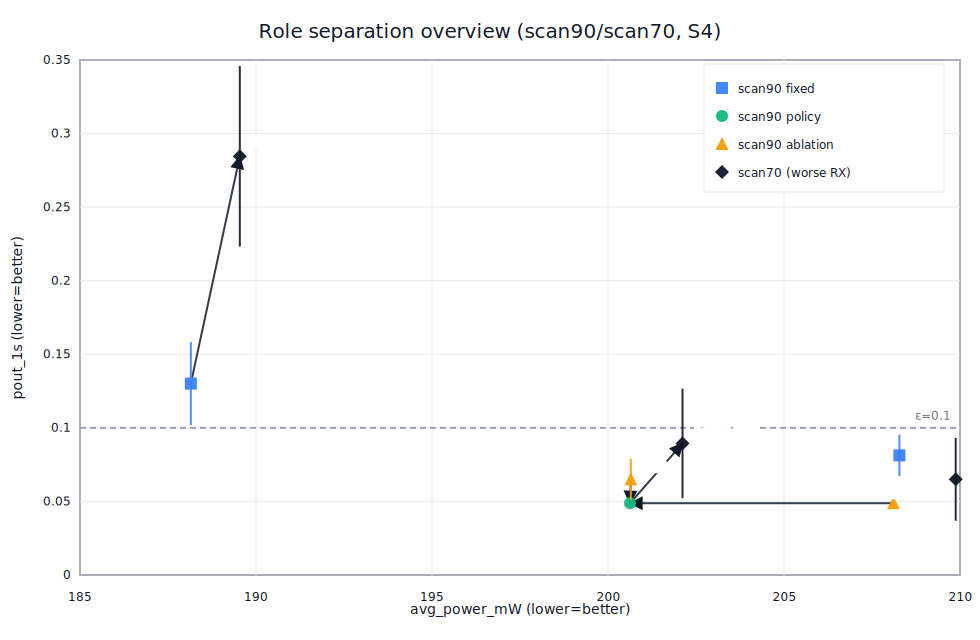
\includegraphics[width=\textwidth,trim=0 0 0 12mm,clip]{figures/fig_role_separation_overview}
  \caption{U/CCSの役割分離(S4)}
  \label{fig:role_separation}
\end{figure*}

図\ref{fig:role_separation}に,固定$\SI{100}{\milli\second}$/固定$\SI{500}{\milli\second}$と方策の関係を,scan90/scan70およびアブレーションを含めて示す(横軸:平均電力,縦軸:$\Pout(\SI{1}{\second})$).

\par
scan90のD2b(S1/S4,各条件$n=6$)では,方策は固定$\SI{100}{\milli\second}$より\SIrange{7.9}{12.6}{\milli\watt}低電力であり,固定$\SI{500}{\milli\second}$より低い$\Pout(\SI{1}{\second})$を示す運用点になり得た(例:S4で固定500が0.146に対し方策は0.069).

\par
受信条件を悪化させたscan70のD3(S4,各条件$n=3$)では,固定$\SI{500}{\milli\second}$が$\Pout(\SI{1}{\second})=0.285\pm0.061$と大きく悪化した一方,方策は$0.089\pm0.037$に抑え,固定$\SI{100}{\milli\second}$($209.9\pm0.5\,\si{\milli\watt}$)より低い平均電力($202.1\pm0.1\,\si{\milli\watt}$)で$\epsout=0.1$を満たした.

\par
さらにscan90/S4のアブレーション(各条件$n=3$)では,U-shuffleは平均電力が$208.1\pm0.3\,\si{\milli\watt}$と固定$\SI{100}{\milli\second}$近傍まで増加し,短間隔への張り付きが増える挙動が確認された.一方でCCS-offは平均電力が方策とほぼ同一(約$200.6\,\si{\milli\watt}$)にもかかわらず,$\Pout(\SI{1}{\second})$が方策の0.0488に対して$0.065\pm0.014$へ悪化した.

\section{考察}
U-shuffle(D4,scan90/S4)では短間隔への張り付きが増加し,平均電力が固定$\SI{100}{\milli\second}$近傍まで戻ったことから,不確実度$U$の時間整合が短間隔滞在量(電力)を規定することが示唆される.一方でCCS-off(D4B,scan90/S4)では,平均電力がほぼ同一のまま$\Pout(\SI{1}{\second})$が悪化したことから,CCSは短間隔滞在量ではなく「短間隔を使うタイミング」によりQoSを改善すると解釈できる.

\par
固定条件の平均電力を$P_{100},P_{500}$とすると,方策の短間隔滞在比率$\rhohundred$は平均電力$P$から
\begin{equation}
  \rhohundred=\frac{P-P_{500}}{P_{100}-P_{500}}
\label{eq:rho_from_power}
\end{equation}
と推定できる.この推定により,省電力効果の支配要因を「sleep設定」ではなく「短間隔滞在量」に帰着でき,制御則設計や学習(Bandit)への拡張時の目的関数設計にも接続できる.

\section{まとめ}
HAR不確実度に基づく2値広告間隔制御が,固定間隔の中間的電力でQoS制約$\Pout(\tau)\le\epsout$を満たす運用点になり得ることを実機で示した.さらに,UとCCSのアブレーションにより,Uは短間隔滞在量(電力),CCSは同電力でのQoS改善を担うことを示唆した.今後は,広告間隔候補の多段化と,制約下で広告間隔を選択する多腕バンディットへ展開する\scite{Auer2002Bandit}.

\vspace{-1mm}
\section*{参考文献}
\printbibliography[heading=none]

\end{document}
